\documentclass[10pt]{article}
\usepackage[top=50pt,bottom=50pt,left=48pt,right=46pt]{geometry}
\usepackage{color}
\usepackage[utf8]{inputenc}
\usepackage{float}
\usepackage[T1]{fontenc}
\usepackage{indentfirst}
\usepackage{amsmath}
\usepackage{graphicx}
\usepackage{hyperref} 
% used for enumerate based on different symbols
% \begin{enumerate}[(a)] e.g.
\usepackage[shortlabels]{enumitem}

% beautifully indenting an environment
% \begin{addmargin}[1em]{2em}
% \end{addmargin}
% args: left margin, right margin
\usepackage{scrextend}

% for centered p columns in tabular environment
% \begin{tabular}{|P{2cm}|P{40mm}|P{4cm}|}
\usepackage{array}
\newcolumntype{P}[1]{>{\centering\arraybackslash}p{#1}}
\newcolumntype{M}[1]{>{\centering\arraybackslash}m{#1}}

% for scaling a tabular table
\usepackage{graphicx}

\usepackage{listings}
% for code writing
% \begin{lstlisting}
% 	code here
% \end{lstlisting}
\lstset{
	breaklines=true,
	tabsize=2,
	basicstyle=\ttfamily,
}


% for comment block
\usepackage{verbatim}

% for debug purposes
% \usepackage{showframe}

% for setting section start value
%\setcounter{section}{2}

% for code writing
% \begin{lstlisting} code here \end{lstlisting}
\usepackage{listings}
\lstset{
	% numbers=left,
	breaklines=true,
	tabsize=2,
	basicstyle=\ttfamily,
	literate={\ \ }{{\ }}1,
	extendedchars=\true
}



\newcommand{\indentitem}{\setlength\itemindent{25pt}}

\newcolumntype{P}[1]{>{\centering\arraybackslash}p{#1}}



% Title Page
\title{Implementation of Databases \\ ~~~ \\ Assignment 3 \\ ~~~ \\ }
\author{
	Participants:\\
	(sorted in last name order)\\
	Ulfet CETIN\\ 
	Shreya KAR\\
	Samuel ROY\\	
}
\date{}


\begin{document}

	\maketitle
	
	\clearpage
	
	\section*{Exercise 3.1 (Tableaux Containment and Minimization)}
	Given are the following tableaux:
	

			
		\begin{figure}[!htb]
			\centering
			\begin{minipage}[t]{0.2\textwidth}
				\begin{table}[H]
				\scalebox{0.9}{
					\begin{tabular}{c c c c}
						T1 	& 		& 		& \\
						\hline
						& a1 	& a2 	&  \\
						\hline
						& b3	& a2	& (R) \\
						& a1	& b4	& (R)\\
						& 5		& b3	& (R)\\
						& b4	& 5		& (R)
					\end{tabular}
				}
				\end{table}
			\end{minipage}
			%
			\begin{minipage}[t]{0.2\textwidth}
				\begin{table}[H]
				\scalebox{0.9}{
					\begin{tabular}{c c c c}
						T2 	& 		& 		& \\
						\hline
						&a1 &a2& \\
						\hline
						&b4 &a2& (R)\\
						&b1 &a2& (R)\\
						&a1 &b3& (R)\\
						&b2 &b4& (R)\\
						&b2 &b1& (R)\\
						&b3 &b2& (R)\\
					\end{tabular}
				}
				\end{table}
			\end{minipage}
			%
			\begin{minipage}[t]{0.2\textwidth}
				\begin{table}[H]
				\scalebox{0.9}{
					\begin{tabular}{c c c c}
						T3 	& 		& 		& \\
						\hline
						&a1& a2&\\
						\hline
						&b3& a2& (R)\\
						&a1& b2& (R)\\
						&b4& b1& (R)\\
						&b1& b2& (R)\\
						&b2& b3& (R)\\
						&b1& b3& (R)\\
					\end{tabular}
				}
				\end{table}
			\end{minipage}
		\end{figure}
		
		\textcolor{red}
		{
			For first question, we have used:\\
		}
		
		Aho, A. V., Sagiv, Y., \& Ullman, J. D. (1979). Efficient optimization of a class of relational expressions. ACM Transactions on Database Systems, 4(4), 435-454. doi:10.1145/320107.320112
		\bigskip
		
		Just to provide you an easier access, here is the link:
		
		\href{url}{http://citeseerx.ist.psu.edu/viewdoc/download?doi=10.1.1.259.3427\&rep=rep1\&type=pdf}
		
		\begin{enumerate}
			\item Find out if T$_{i}$ $\subseteq$ T$_{j}$ i.e., T$_{i}$  T$_{j}$ for i $\neq$ j, i, j $\in$ \{1, 2, 3\}.
			
			We have gone through all possible mappings from T$_{i}$ $\subseteq$ T$_{j}$ i.e., T$_{i}$  T$_{j}$ for i $\neq$ j, i, j $\in$ \{1, 2, 3\}.
			
			Yet, we only found that T1 $\subseteq$ T2 holds.
			
			
			\vspace{3em}
			\begin{minipage}[t]{.98\linewidth}
				\begin{minipage}[t]{0.55\linewidth}
					
					Here is the mapping.\\
					\bigskip
					
					\scalebox{1.5}{
					
					\begin{tabular}{|ccc|}
						
						\hline
						T2 	& 	to	& 	T1 \\
						\hline
						a1 & $\rightarrow$ & a1 \\
						\hline
						a2 & $\rightarrow$ & a2 \\
						\hline
						b1 & $\rightarrow$ & b3 \\
						\hline
						b2 & $\rightarrow$ & 5 \\
						\hline
						b3 & $\rightarrow$ & b4 \\
						\hline
						b4 & $\rightarrow$ & b3 \\
						\hline
					\end{tabular}
					}
				\end{minipage}
				\quad
				\begin{minipage}[t]{0.4\linewidth}
					Here is mapped T2.\\
					
					\begin{table}[H]
						\scalebox{1.2}{
							\begin{tabular}{c c c c}
								T2\_mapped 	& 		& 		& \\
								\hline
								&a1& a2&\\
								\hline
								&b3& a2&\\
								&b3& a2 \\
								&a1& b4\\
								&5& b3\\
								&5& b3\\
								&b4& 5\\
								
							\end{tabular}
						}
					\end{table}
				\end{minipage}
			\end{minipage}
			
			\bigskip			
			
			\item Write down the minimal tableau for T$_{i}$ , i $\in$ {1, 2, 3}.
		\end{enumerate}
		
	\begin{figure}[!htb]
		\centering
		\begin{minipage}[t]{0.3\textwidth}
			\begin{table}[H]
				\centering
				\scalebox{0.9}{
					\begin{tabular}{c c c c}
						T1 	& 		& 		& \\
						\hline
						& a1 	& a2 	&  \\
						\hline
						& b3	& a2	& (R) \\
						& a1	& b4	& (R)\\
						& 5		& b3	& (R)\\
						& b4	& 5		& (R)
					\end{tabular}
				}
				
				\bigskip
			\end{table}
		\end{minipage}
		%
		\begin{minipage}[t]{0.3\textwidth}
			\begin{table}[H]
				\centering
				\scalebox{0.9}{
					\begin{tabular}{c c c c}
						T2 	& 		& 		& \\
						\hline
						&a1 &a2& \\
						\hline
						&b1 &a2& (R)\\
						&a1 &b3& (R)\\
						&b2 &b1& (R)\\
						&b3 &b2& (R)\\
					\end{tabular}
				}
				\bigskip
			\end{table}
		\end{minipage}
		%
		\begin{minipage}[t]{0.3\textwidth}
			\begin{table}[H]
				\centering
				\scalebox{0.9}{
					\begin{tabular}{c c c c}
						T3 	& 		& 		& \\
						\hline
						&a1 &a2& \\
						\hline
						&b3 &a2& (R)\\
						&a1 &b2& (R)\\
						&b4 &b1& (R)\\
						&b1 &b2& (R)\\
						&b2 &b3& (R)\\
						&b1 &b3& (R)\\
					\end{tabular}
				}
				
			
			\end{table}
		\end{minipage}
	\end{figure}
	
	\begin{figure}[!htb]
		\centering
		\begin{minipage}[t]{0.29\textwidth}
			T1 is already a minimal Tableau.
		\end{minipage}
		%
		\begin{minipage}[t]{0.05\textwidth}
			\hspace{0.01mm}
		\end{minipage}
		%
		\begin{minipage}[t]{0.29\textwidth}
			Mapping b4 $\rightarrow$ b1, this is the minimal Tableau
		\end{minipage}
		%
		\begin{minipage}[t]{0.05\textwidth}
			\hspace{0.01mm}
		\end{minipage}
		%
		\begin{minipage}[t]{0.29\textwidth}
			 T3 is already a minimal Tableau.
		\end{minipage}
	\end{figure}
		
	
	
	\clearpage


	\section*{Exercise 3.2 (Quant Graphs)}
		Given is the Chinook database schema (see Assignment 1).
		
		\begin{enumerate}
			\item Specify the following queries in TRC and draw the corresponding quant graphs, subsequently.
			Determine for each graph, if it contains a cycle. Explain in your own words what this means
			for the query.	
			
				\begin{enumerate}[(a)]
					\item EmployeeId and LastName of employees who have supported at least two different
					customers living in the same city.
					
					\begin{minipage}[t]{.98\linewidth}
						\begin{minipage}[t]{0.55\linewidth}
							
							TRC\\
							$
							\{ <e.EmployeeId>, <e.LastName> | e \in Employee
							\\ \hspace*{2em}(
							\\ \hspace*{4em}\exists c1 \in Customer \; \exists c2 \in 	Customer
							\\ \hspace*{4em}(
							\\\hspace*{6em} c1.City=c2.City \Lambda
							\\ \hspace*{6em}c1.SupportRepId =c2.SupportRepId \Lambda
							\\ \hspace*{6em}c1.SupportRepId= e.EmployeeId
							\\\hspace*{4em})
							\\ \hspace*{2em})
							\\ \}
							$
						\end{minipage}
						\quad
						\begin{minipage}[t]{0.4\linewidth}
							\vspace{-2ex}
							\hspace{-2ex}
							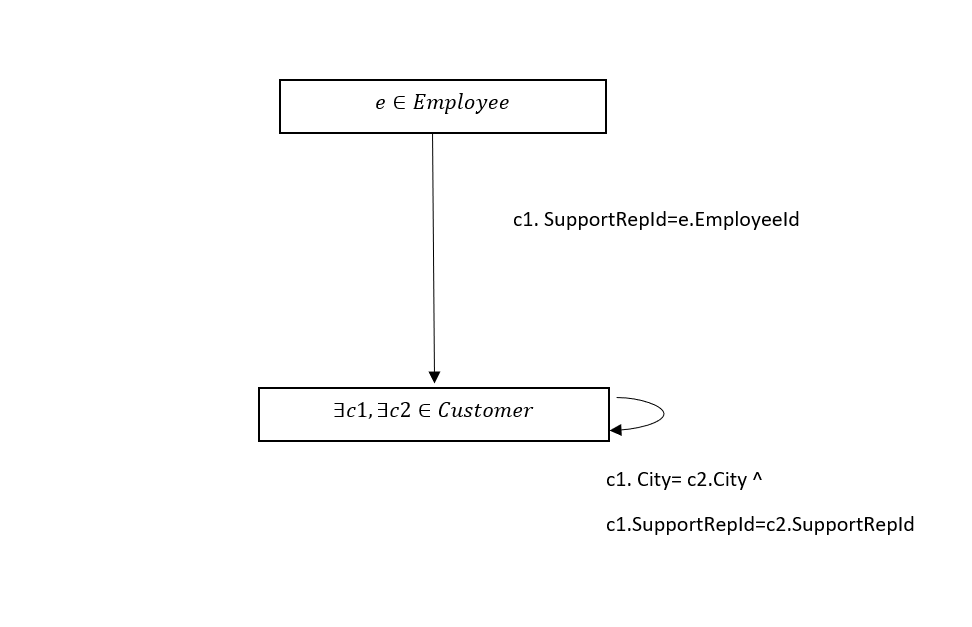
\includegraphics[width=1.1\linewidth]{q1.PNG}
						\end{minipage}
					\end{minipage}
					
					\bigskip
					This Query contains a cycle as there exists a predicate cycle from relation Customer to the node 					 itself. The problem with a cyclic quant graph is that There is no sequence of semijoin operators that compute the correct result for arbitrary database states.
					However, it doesn't make a difference in particular query as the semijoin between the same relation (Customers) will yield the same result. In other words, the order here is trivial to compute the intermediate result as the same relation is involved.
					
				
					\bigskip
					
					\item Track name and composer of all tracks, which are from the genre “Rock” and where
					the artist is also the composer.
						Solution:
						
						\begin{minipage}[t]{.98\linewidth}
							\begin{minipage}[t]{0.55\linewidth}
								TRC:
								$
								\\
								\{ <t.Name>,<t.Composer> | t \in Track
								\\\hspace*{2em}(
								\\ \hspace*{4em} \exists a \in Album
								\\\hspace*{4em} \exists a1 \in Artist
								\\ \hspace*{4em}\exists g \in Genre
								\\\hspace*{4em}(
								\\ \hspace*{8em} t.AlbumId = a.AlbumId \Lambda
								\\ \hspace*{8em}a.ArtistId = a1.ArtistId \Lambda
								\\ \hspace*{8em}t.Genre= g.Genre \Lambda
								\\ \hspace*{8em}t.Composer = a1.Name \Lambda
								\\ \hspace*{8em}t.Genre = "Rock"
								\\\hspace*{4em})
								\\\hspace*{2em})
								\\	\}
								$
							\end{minipage}
							\quad
							\begin{minipage}[t]{0.4\linewidth}
								\vspace{-2ex}
								\hspace{-2ex}
								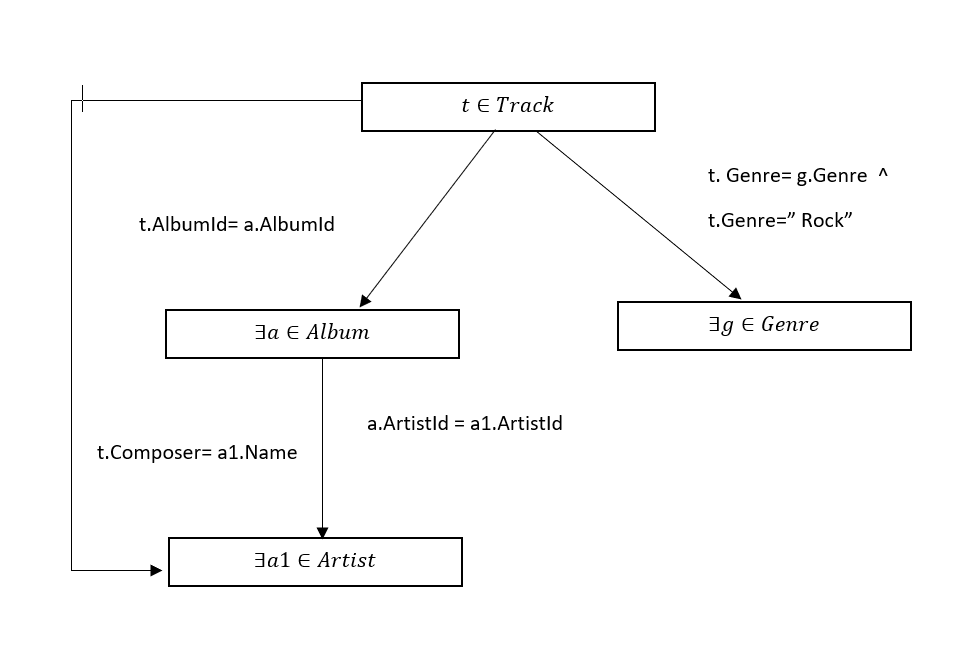
\includegraphics[width=1.0\linewidth]{q2.PNG}
							\end{minipage}
						\end{minipage}
						
					\bigskip
					This query contains a cycle as there exists a predicate cycle. What it means is that there is no 					 sequence of semijoin operators that compute the correct intermediate result for given relations 						Track,Album and Artist.It also implies that there are certain intermediate DB states where no possible sequence of operands can achieve a
                    reduction of the involved range relations.
                    \\i.e. Rel1 semijoin with Rel2 where 
                    $ Rel1,Rel2 \in \{Track,Album,Artist\} $
                    will always yield Rel1 as result
                    
					
				\end{enumerate}
		\end{enumerate}

	\clearpage

	\section*{Exercise 3.3 (Join Implementations)}
		
		Let relations R and S have the following properties:
		\begin{itemize}
			\item R has 10,000 tuples and has 10 tuples per page
			
			\item S has 2000 tuples and also has 10 tuples per page
			
			\item Both the relations are stored as simple heap files and neither relation has any indexes built
			on it.
		\end{itemize}
		
		The total number of buffers available is 52.
		Now considering the join R $\bowtie _{R.a=S.b}$ S assuming that attribute b on relation S is the primary
		key for S, answer the following questions: (The cost of writing out the result should be uniformly
		ignored.)
		
		\begin{enumerate}
			\item Calculate the I/O requirements of a page-oriented simple nested loop join.
				Solution:
			\\M=number of pages for relation R
			  = 10000/10
			  =1000
			\\N= number of pages for relation S
			  = 2000/10
			  =200
			  \\I/0 costs of page oriented Simple nested loop join (taking R as outer relation)= M+M*N
			        \\=1000+1000*200
			       \\ =2,01,000
			 \\I/0 costs of page oriented Simple nested loop join(taking S as outer relation)= N+N*M
			        \\=200+200*1000
			       \\ =2,00,200
			\bigskip
			
			
			\item Calculate the I/O requirements of a block nested loop join.
			Solution:
			    \\B=52
			    \\I/O requirements of Block Nested Loop join (taking R as outer relation)=M+[M/(B-2)]*N
			    \\=1000+[1000/(52-2)]*200
			    \\=1000+20*200
			    \\=5000
			     \\I/O requirements of Block Nested Loop join (taking S as outer relation)=N+[N/(B-2)]*M
			    \\=200+[200/(52-2)]*1000
			    \\=200+4*1000
			    \\=4200
		\end{enumerate}

	\clearpage

	\section*{Exercise 3.4 (Cost Estimation)}
	
		\begin{enumerate}
			\item Consider the following relations and the number of distinct values for the different attributes
			V (R, a). Each of the relations has a size of 1000 tuples. Determine an optimal order for
			joining all three relations. For each intermediate step determine the sizes of the results in
			terms of tuples. The cost of each plan is the sum of all intermediate result sizes. Select the
			best plan based on your results.
			
			\begin{table}[H]
				\centering
				\scalebox{0.9}{
					\begin{tabular}{c c c}
						R(a,b) & S(b,c) & T(c,d)\\
						\hline
						V(R,a) = 100 	& 				& \\
						V(R,b) = 200	& V(S,b)=100 	& \\
										& V(S,c)=500	& V(T,c)=20\\
										&				& V(T,d)=50 \\
						\hline
					\end{tabular}
				}
			\end{table}
		
	The result size of joining relations R(X,Y) and S(Y,Z) can be approximated by:
	
	\[ T=\frac{T(R) * T(S) }{max(V(R,Y),V(S,Y))} \]
	
	(R $\bowtie$ S) $\bowtie$ T , R $\bowtie$ (S $\bowtie$ T) are the possible plans:\\\\
	R(a,b) with T(R)=1000 and V(R,b)=200\\
	S(b,c) with T(S)=1000 and V(S,b)=100 and V(S,c)= 500\\
	T(c,d) with T(T)=1000 and V(T,c)=20\\
	
	Size and Cost Calculation for(R $\bowtie$ S) $\bowtie$ T:\\
	
	\[ T(R \bowtie S)=\frac{T(R) * T(S) }{max(V(R,b),V(S,b))} \] 	\[ =\frac{1000 * 1000 }{200} \] \[ =5000 \] \\
	\[ T(R \bowtie S) \bowtie T=\frac{T(R \bowtie S) * T(T) }{max(V(R \bowtie S,c),V(T,c))} \] 	\[ =\frac{5000 * 1000 }{500} \] \[ =10000 \] 
	
	Total Cost for(R $\bowtie$ S) $\bowtie$ T : 10000+5000=15000\\
	
		Size and Cost Calculation for R $\bowtie$ (S $\bowtie$ T):\\
	
	\[ T(S \bowtie T)=\frac{T(S) * T(T) }{max(V(S,c),V(T,c))} \] 	\[ =\frac{1000 * 1000 }{500} \] \[ =2000 \] \\
	\[ T(S \bowtie T) \bowtie R=\frac{T(S \bowtie T) * T(R) }{max(V(S \bowtie T,b),V(T,b))} \] 	\[ =\frac{2000 * 1000 }{200} \] \[ =10000 \] 
	
	Total Cost for(R $\bowtie$ S) $\bowtie$ T : 10000+2000=12000
	
	Best plan is R $\bowtie$ (S $\bowtie$ T)

			\item Consider the following relational schema and SQL query. The schema captures information
			about employees, departments, and finances (organized on a per department basis).
			
				\bigskip
				\begin{addmargin}[0.30\textwidth]{4em}
					Suppliers(\underline{sid}, sname, city)\\
					Supply(\underline{sid, pid})\\
					Parts(\underline{pid}, pname, price)
				\end{addmargin}
				
				\begin{lstlisting}
					SELECT P.pname
					FROM Suppliers S , Parts P , Supply Y
					WHERE S.sid=Y.sid AND Y.pid=P.pid AND
					S.city= ’ Aachen ’ AND P.price <= 200 AND
					Y.pid < 800
				\end{lstlisting}
				
				\begin{enumerate}[(a)]
					\item Identify a relational algebra tree (or a relational algebra expression if you prefer) that
					reflects the order of operations a decent query optimizer would choose (applying the
					heuristics selection before join, and projections are done as many and as early as possible).\\
					
					$ \rho(suppliersInAachen,
					\Pi_{sid}( \sigma_{city="Aachen"} Suppliers) ) $\\
					
					$ \rho(suppliedTo, 
					\Pi_{pid}( suppliersInAachen \bowtie (\sigma_{pid < 800}Supply)) ) $\\
					
					$\Pi_{pname}( suppliedTo \bowtie (\Pi_{pid, pname}(\sigma_{price <= 200}Parts)) )$
					\bigskip
					
					\item What indexes for single attributes might be of help in processing this query? Should it
					be clustered or unclustered indexes, using hash tables or B+ trees?
					\bigskip
					
					There are three where we do selection. The rest of the fields in WHERE clause, those will be handled with join operations.
					
					$\lbrace$ Suppliers.city, Supply.pid, Part.price $\rbrace$
					
					\bigskip
					
					\begin{table}[H]
						\centering
						\scalebox{0.9}{
							\begin{tabular}{|c|c|p{11cm}|}
								\hline
								Field Name & Clustered or Unclustered & Hash Table or B+ Tree \\
								\hline
								Suppliers.city & Unclustered & Both hash table and B+ tree would work: \\
								 &  & 1) based on implementation, hash table may work bad if bucket approach is not used \\
								 &  & 2) B+ tree would work better, as records having their city field as "Aachen" will be placed consecutively if data records are stored (instead of data entries) \\
								\hline
								Supply.pid & Clustered & Both hash table and B+ tree would work: \\
								&  & BUT B+ tree would work better most probably.\\
								&  & This answer is also based on how specific DB system works: if hash table finds one entry and goes above and below in the corresponding data record file to find the rest of the records, it is also good, too. But if each and every record will be tracked from its data entry in the hash table, assuming there is no caching, there will be too many read I/O operation, undermining the effort.  \\
								\hline
								Part.price & Unclustered & Both hash table and B+ tree would work: \\
								&  & 1) based on implementation, hash table may work bad if bucket approach is not used \\
								&  & 2) B+ tree would work better, as records having their city field as "Aachen" will be placed consecutively if data records are stored (instead of data entries) \\
								\hline
							\end{tabular}
						}
					\end{table}
					
					
					\bigskip
					
					\item Suppose that the following additional information is available: The system’s statistics
					indicate that there are suppliers from 100 cities, and part prices range from 1 to 1000
					Euros. All attribute values are uniformly distributed and each id has been created in
					numerical order without any records deleted so far. There are a total of 400 suppliers,
					2.000 parts, and 200.000 entries in the Supply relation in the database.
					For each of the query’s base relations (Supply, Suppliers, Parts) estimate the number of
					tuples that would be initially selected from that relation if all of the non-join predicates
					on that relation were applied to it before any join processing begins.
					
					\bigskip
					Here are the estimations:
					
					\begin{itemize}
						\item $( \sigma_{city="Aachen"} Suppliers)$\\
						\#Entries without Selection = 400, \\
						\#Entries with Selection = 400 * $\frac{1}{100}$ = 4\\
						
						\item $(\sigma_{pid < 800}Supply) $\\
						\#Entries without Selection = 200000, \\
						\#Entries with Selection = 800,\\
						(note that pid is the primary key, and it is noted in the question that each ID is created in numerical order and none has been deleted)\\
						
						\item $(\sigma_{price <= 200}Parts)$\\
						\#Entries without Selection = 2000, \\
						\#Entries with Selection = 2000 * $\frac{200 - 0}{1000-0}$ = 400\\
					\end{itemize}
					
					
					\bigskip
					
					\item Based on the results for (c), which pair of relations should be joined first?
					
					As we want to avoid cross product as because of its cost, we want to look at which join routes are possible:
					
					\begin{itemize}
						\item (Suppliers $\bowtie$ Supply)\\
						Selection-applied Suppliers relation has 4 entries,\\
						Selection-applied Supply relation has 800\\
						
						\item (Supply $\bowtie$ Parts)
						Selection-applied Supply has 800 entries,\\
						Selection-applied Parts relation has 2000 entries.\\
					\end{itemize}
					
					Based on those numbers, it will be better to do (Suppliers $\bowtie$ Supply) join operation first; as it will reduce the number of 800 Supply entries to a hopefully far less qualifying matches of entries.\\
					Instead of comparing 800 entries with 2000 entries in (Supply $\bowtie$ Parts), doing the first will make things run faster.\\
					
					So, the answer is (Suppliers $\bowtie$ Supply) as it is expected to lead to a greater reduction in the number of operations.
				\end{enumerate}
		\end{enumerate}
		
\end{document} 
